%卒論概要テンプレート ver. 4.0

\documentclass[uplatex,twocolumn,dvipdfmx]{jsarticle}
\usepackage[top=22mm,bottom=22mm,left=22mm,right=22mm]{geometry}
\setlength{\columnsep}{11mm}
\usepackage[T1]{fontenc}
\usepackage{txfonts}
\usepackage[expert,deluxe]{otf}
\usepackage[dvipdfmx,hiresbb]{graphicx}
\usepackage[dvipdfmx]{hyperref}
\usepackage{pxjahyper}
\usepackage{secdot}





%タイトルと学生番号,名前だけ編集すること
\title{\vspace{-5mm}\fontsize{14pt}{0pt}\selectfont Twitterにおけるデマ拡散のシミュレーション}
\author{\normalsize プロジェクトマネジメントコース 矢吹研究室 1442043 川崎貴雅}
\date{}
\pagestyle{empty}
\begin{document}
\fontsize{10.5pt}{\baselineskip}\selectfont
\maketitle



%以下が本文
\section{序論}\label{序論}

Twitterはリアルタイムな情報を手軽に多くのユーザへと伝播できるため社会に影響を与えている.\#MeTooというハッシュタグの投稿により性的被害やセクハラについて考えるきっかけが,世界中に広がった事が挙げられる.
しかし悪い影響を与えてしまう場合もある.例えば東日本大震災時のライオンの脱走や北朝鮮のミサイルの目撃デマが挙げられる.このようなツイートの拡散をシミュレーションで再現することを試みる.
本研究ではTwitterのデマ拡散をシミュレーションで再現することができるかの調査を行う.

\section{目的}

本研究では現実のデマ拡散に近い状況を再現できるシミュレーションの開発することである.

\section{手法}

デマの拡散をシミュレートするためには,ユーザ同士のネットワーク作成,つぶやきの頻度,RTの頻度を求めることが必要なため,以下の手順で行う.
\begin{enumerate}
\item ツイートの拡散する様子をシュミレートする手法を確立するために,ランダムグラフでのRTシミュレーションを試みる\cite{netto}.
\item TwitterAPIを用いて50万人のユーザから1日のツイート数取得を行い,それをもとに1日あたりのツイート数の分布を出す.
\item ユーザから1日のRT数の取得を行い,分布を出す.
\item ネットワークの作成のためユーザーのォロー数の平均を出す.
\end{enumerate}

\section{結果}

Twitterユーザ50万人分のデータを使って,1日あたりのツイート数の確率分布を描くと図\ref{ツイートの分布}のようになる.これによくフィットする関数を探索すると$C/(1+\exp(t-1))$($C$は定数)であった.全確率が1になるように$C=1/\log(1+e)$とし,ツイート数の期待値を求めると約$1.38$となった.またグループ構築にランダムグラフを使ったツイート拡散のシュミレート手法も確立できた.しかし1日あたりのRT数の分布と1ユーザのフォロー人数の平均が出せなかったため現実的なシミュレーションを行うことはできなかった.

\begin{figure}[htb]
\centering
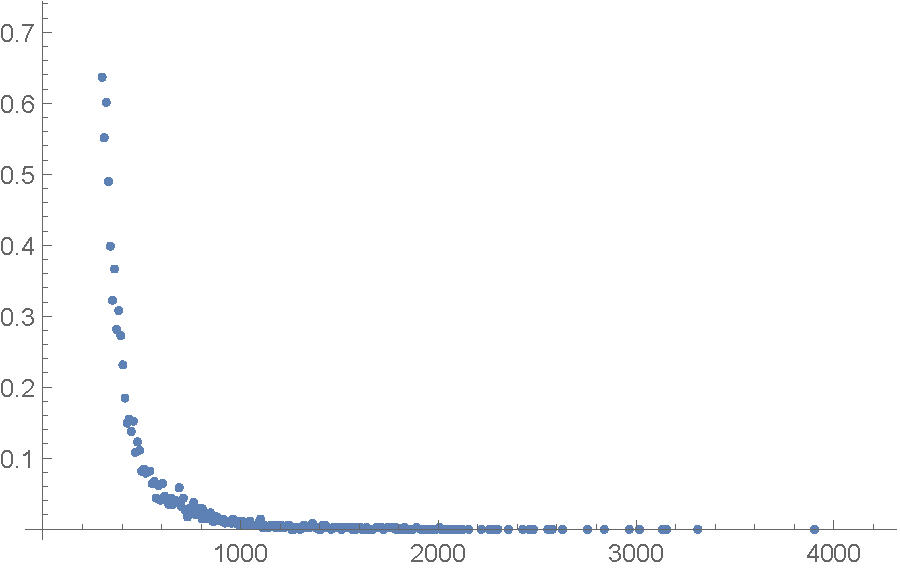
\includegraphics[width=77mm,clip]{tweets.pdf}
\caption{1日のツイート数に対する割合}\label{ツイートの分布}
\end{figure}

\section{考察}

10人でのシミュレーションのメンバ全てがツイートを確認できるようになるのは互いに繋がってる確率が0.5でRTする確率が0.6のときである.この場合フォローしている人間は5人で,その中で3人の人間がRTをすると考えられる.

\section{結論}

本研究では,1日のツイート数の分布とツイート拡散のシュミレートをする手法の確立を行った.その結果1日のツイート数の分布確認,ツイートの拡散シミュレートの手法の確立が行えた.この結果に1日あたりのRT数の分布と1ユーザのフォロー人数の平均が取得できれば現実に近いシミュレーションを行うことが期待できる.

\bibliographystyle{junsrt}
\bibliography{biblio}%「biblio.bib」というファイルが必要.

\end{document}
